\section{Résultats de Hoppe et Rahmat-Samii}

Cette section référence les résultats de \cite{hoppe_impedance_1995}


La figure \ref{fig:annex:hoppe:p62} représente la partie imaginaire du symbole de l'opérateur d'impédance tel que \( \hat{\vE}_t(r_1,n,k_z) = \hat{\mZ}(n,k_z) \hat{\vH}(r_1,n,k_z) \) où $\vH$ n'est pas normalisé par \gls{phy-eta_zero} pour un cylindre.

\begin{figure}[h!tb]
    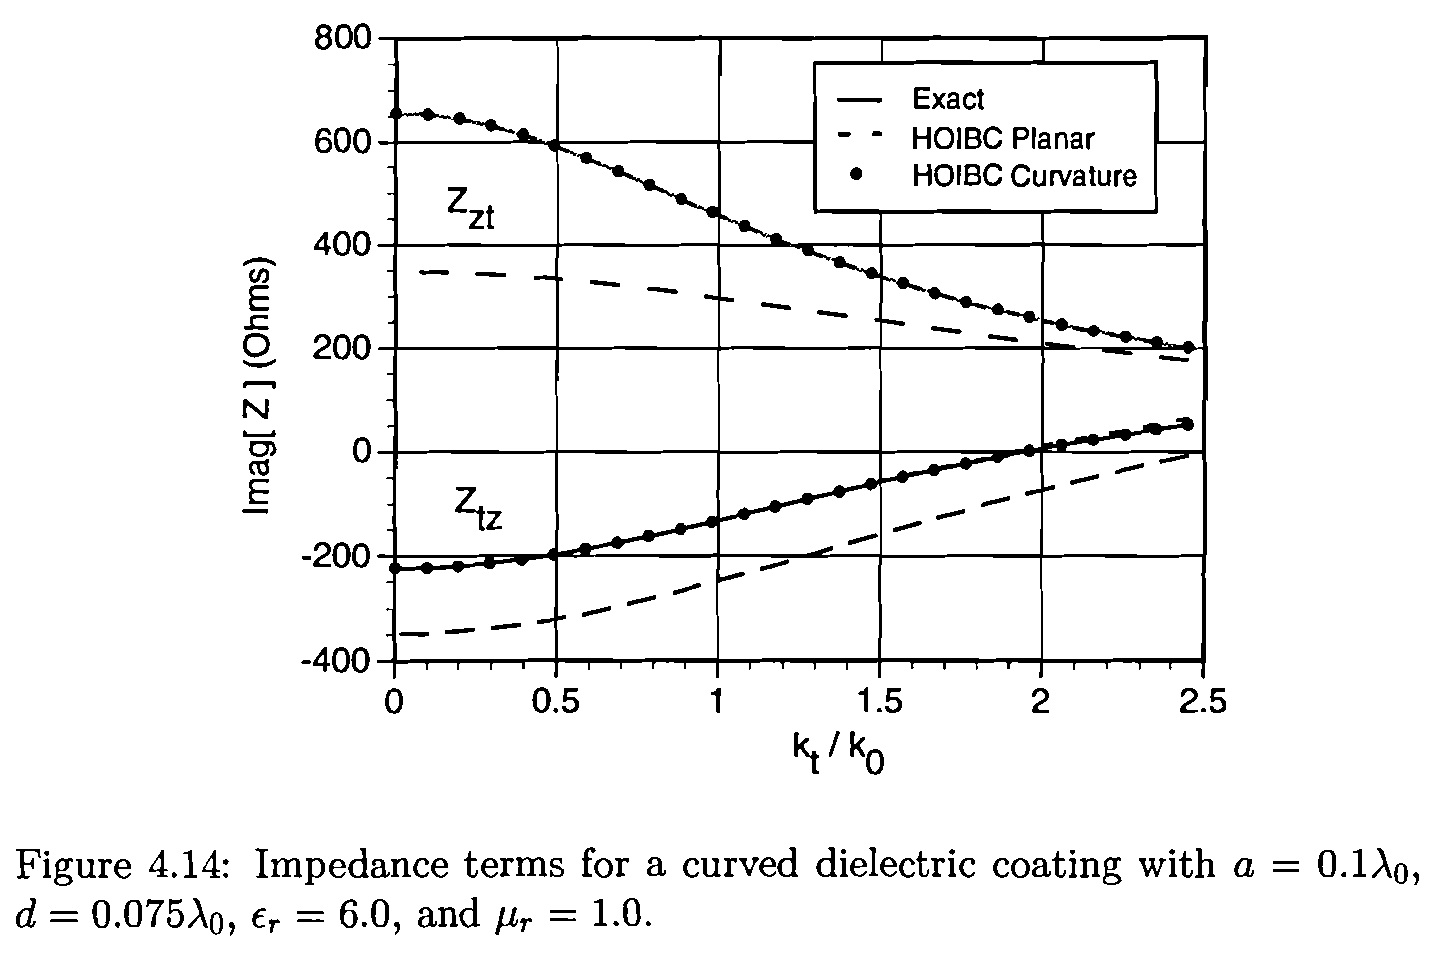
\includegraphics[width=0.99\textwidth]{images/hoppe/p62_imp_cylindre.png}
    \caption{Courbes de la page 62 de Hoppe Rahmat-Samii 1995}
    \label{fig:annex:hoppe:p62}
\end{figure}

Ainsi, \(Z_{zt}\) correspond à \(-\eta_0\hat{\mZ}_{11}\) (TM) et \(Z_{tz}\) correspond à \(\eta_0\hat{\mZ}_{22}\) (TE) de la figure \ref{fig:imp_fourier:cylindre:hoppe_p62}.